% =====================================================================
% Affiche -- Probleme 1, GEI723 (Automne 2026) : locomotion hexapode
% Compilation : xelatex affiche ; bibtex affiche ; xelatex affiche ; xelatex affiche
%   (ou latexmk -xelatex affiche.tex ; sur Overleaf : compilateur XeLaTeX)
% Figures : figures/*.pdf, produites par Code/poster_figs.py et Code/annexe_figs.py
% =====================================================================
\documentclass[20pt, a0paper, portrait, margin=0mm, innermargin=24mm,
  colspace=19mm, subcolspace=0mm, blockverticalspace=6mm]{tikzposter}
% =====================================================================
% Style commun de l'affiche et de l'annexe (tikzposter, A0 portrait).
% Compiler avec XeLaTeX (ou LuaLaTeX) : les polices IBM Plex sont dans fonts/.
% =====================================================================
\usepackage{fontspec}
\usepackage{polyglossia}
\setdefaultlanguage{french}
\usepackage{graphicx}
\usepackage{booktabs}
\usepackage{array}
\usepackage{tabularx}
\usepackage{amsmath}
\usepackage{enumitem}
\usetikzlibrary{arrows.meta}

% ---------------------------------------------------------------- polices
\setmainfont{IBMPlexSans}[Path=fonts/, Extension=.ttf, UprightFont=*-Regular,
  BoldFont=*-SemiBold, ItalicFont=*-Italic]
\setsansfont{IBMPlexSans}[Path=fonts/, Extension=.ttf, UprightFont=*-Regular,
  BoldFont=*-SemiBold, ItalicFont=*-Italic]
\setmonofont{IBMPlexMono}[Path=fonts/, Extension=.ttf, UprightFont=*-Regular,
  BoldFont=*-SemiBold]
\newfontfamily\condensed{IBMPlexSansCondensed}[Path=fonts/, Extension=.ttf,
  UprightFont=*-Bold, BoldFont=*-Bold]
\newfontfamily\plexbold{IBMPlexSans}[Path=fonts/, Extension=.ttf, UprightFont=*-Bold]

% ---------------------------------------------------------------- couleurs
\definecolor{encre}{HTML}{16161A}
\definecolor{encre2}{HTML}{2C2C33}
\definecolor{gris}{HTML}{4A4A52}
\definecolor{filet}{HTML}{D9D6CE}
\definecolor{fond}{HTML}{FBFAF7}
\definecolor{carton}{HTML}{FFFFFF}
\definecolor{bordure}{HTML}{E4E2DC}
\definecolor{bleu}{HTML}{2A78D6}
\definecolor{orange}{HTML}{EB6834}
\definecolor{excit}{HTML}{3A3A42}
\definecolor{inhib}{HTML}{C2410C}
\definecolor{ambre}{HTML}{8A6D00}

% ---------------------------------------------------------------- theme tikzposter
\definecolorstyle{Affiche}{}{%
  \colorlet{backgroundcolor}{fond}
  \colorlet{framecolor}{fond}
  \colorlet{titlefgcolor}{encre}
  \colorlet{titlebgcolor}{fond}
  \colorlet{blocktitlebgcolor}{fond}
  \colorlet{blocktitlefgcolor}{encre}
  \colorlet{blockbodybgcolor}{fond}
  \colorlet{blockbodyfgcolor}{encre}
  \colorlet{innerblocktitlebgcolor}{fond}
  \colorlet{innerblocktitlefgcolor}{encre}
  \colorlet{innerblockbodybgcolor}{fond}
  \colorlet{innerblockbodyfgcolor}{encre}
  \colorlet{notefgcolor}{encre}
  \colorlet{notebgcolor}{carton}
  \colorlet{notefrcolor}{bordure}
}
\tikzposterlatexaffectionproofoff
\usecolorstyle{Affiche}
\usebackgroundstyle{Empty}
\usetitlestyle{Empty}
\useblockstyle{Minimal}
\defineblockstyle{Affiche}{titlewidthscale=1, bodywidthscale=1, titleleft,
  titleoffsetx=0pt, titleoffsety=0pt, bodyoffsetx=0pt, bodyoffsety=0pt,
  bodyverticalshift=0pt, roundedcorners=0, linewidth=0pt,
  titleinnersep=0mm, bodyinnersep=0mm}{}
\useblockstyle{Affiche}

% ---------------------------------------------------------------- commandes
% Titre de section numerote : \titre{01}{Contexte et objectifs}
\newcommand{\titre}[2]{{\condensed\fontsize{36pt}{40pt}\selectfont
  {\ttfamily\bfseries\color{bleu}#1}\hspace{0.5em}#2}\par\vspace{3mm}}
% Bandeau de partie, pleine largeur
\newcommand{\bandeau}[1]{\noindent{\ttfamily\bfseries\fontsize{20pt}{24pt}\selectfont\addfontfeature{LetterSpace=8}#1}%
  \hspace{1em}\leaders\hrule height 1.2mm\hfill\null}
% Legende de figure : \legende{Fig. 1 --- Titre.}{Texte}
\newcommand{\legende}[2]{\par\vspace{2mm}{\fontsize{17pt}{23pt}\selectfont\color{encre2}\textbf{#1} #2\par}\vspace{4mm}}
% Numero de piece cercle
\newcommand{\num}[1]{\tikz[baseline=(n.base)]\node[circle, draw=encre, line width=0.4mm, inner sep=0.6mm, font=\fontsize{13pt}{13pt}\selectfont\bfseries] (n) {#1};\ }
% Encadre blanc
\newcommand{\encadre}[1]{\noindent\colorbox{carton}{\fcolorbox{bordure}{carton}{\parbox{\dimexpr\linewidth-2\fboxsep-1.6pt-2\fboxrule\relax}{\raggedright #1}}}}
\newcommand{\code}[1]{\texttt{#1}}
\newcommand{\petit}{\fontsize{18pt}{24.5pt}\selectfont}
\newcommand{\corps}{\fontsize{19.5pt}{27pt}\selectfont}
\setlength{\fboxsep}{5mm}
\setlength{\fboxrule}{0.6mm}
\setlength{\parindent}{0pt}
\setlength{\parskip}{3mm}
\setlist{nosep, leftmargin=0pt, labelsep=0pt, itemsep=3mm}
\renewcommand{\arraystretch}{1.25}
\setlength{\heavyrulewidth}{0.6mm}
\setlength{\lightrulewidth}{0.3mm}

% Schemas TikZ
\tikzset{
  carte/.style={rectangle, rounded corners=1.6mm, line width=0.6mm, align=center, inner sep=1mm},
  pill/.style={rounded corners=8mm},
  etiq/.style={inner sep=0pt, text=gris},
  excitl/.style={draw=excit, line width=0.8mm},
  inhibit/.style={draw=inhib, line width=0.8mm},
  bande/.style={draw=bordure!80!gris, dash pattern=on 3mm off 2.5mm, line width=0.6mm, rounded corners=5mm, fill=bordure!35!fond},
}

% Motif raster du CPG (une barre bleue, une orange, periode 197 ms)
\newcommand{\raster}[1]{%
  \begin{tikzpicture}
    \foreach \i in {0,...,15} {
      \fill[bleu, rounded corners=0.4mm] (\i*5.2,0) rectangle ++(0.19,#1);
      \fill[orange, rounded corners=0.4mm] (\i*5.2+2.6,0) rectangle ++(0.19,#1);
    }
  \end{tikzpicture}}


\begin{document}

% ------------------------------------------------------------------ en-tete
\settitle{\begin{minipage}{\linewidth}\raggedright%
  {\ttfamily\fontsize{17pt}{20pt}\selectfont\color{gris}
  GEI723 — NEUROSCIENCES COMPUTATIONNELLES · PROBLÈME 1 · AUTOMNE 2026\hfill
  UNIVERSITÉ DE SHERBROOKE · DÉP. DE GÉNIE ÉLECTRIQUE ET GÉNIE INFORMATIQUE\par}
  \vspace{6mm}
  {\condensed\fontsize{78pt}{82pt}\selectfont Locomotion hexapode par un réseau de neurones à décharges\par}
  \vspace{5mm}
  {\fontsize{25pt}{31pt}\selectfont\color{encre2} Un métronome de deux neurones, des interrupteurs « ET » et des capteurs : de la marche commandée à la marche pseudo-autonome\par}
  \vspace{6mm}
  {\fontsize{27pt}{32pt}\selectfont\bfseries Raphaël Barrette · Émile Jacques-Tighe}\hfill
  \parbox[b]{0.55\linewidth}{\raggedleft\itshape\fontsize{16pt}{20pt}\selectfont\color{gris}
  Nous attestons que nous sommes les auteurs du présent travail et que tout ce qui a été emprunté est attribué à sa source et proprement cité.}\par
  \vspace{6mm}

\end{minipage}}
\maketitle[width=\dimexpr\textwidth-48mm\relax, titletotopverticalspace=20mm, titletoblockverticalspace=12mm, innersep=0mm]

% ------------------------------------------------------------------ bande A
\begin{columns}
\column{0.333}
\block{}{\raggedright%
  \titre{01}{Contexte et objectifs}
  {\fontsize{18.5pt}{26pt}\selectfont Chez l'animal, un réseau de la moelle épinière, le \textbf{générateur central de rythme (CPG)}, produit seul l'alternance des pas : les centres supérieurs ne fixent que la vitesse et la direction, et les perceptions modifient ce rythme sans le remplacer \cite{otis2004}. Nous appliquons ce principe à un hexapode : des neurones à décharges codent les \textbf{instants} où chaque commande de patte est émise.\par}
  \vspace{6mm}
  \begin{minipage}[t]{0.485\linewidth}\encadre{\petit\textbf{Partie I · commandes à la main}\par\vspace{2mm}
    Ligne droite · marche avant · marche arrière · variation de vitesse · rotation sur place · cercle · 20 à 200 paires de pattes}\end{minipage}\hfill
  \begin{minipage}[t]{0.485\linewidth}\encadre{\petit\textbf{Partie II · pseudo-autonome}\par\vspace{2mm}
    Flanc droit → tourner à gauche · flanc gauche → à droite · face → reculer · heurté derrière → accélérer · comportements réglables · 20 à 200 paires}\end{minipage}
}
\column{0.333}
\block{}{\raggedright%
  \titre{02}{Un seul modèle de neurone}
  \encadre{%
    {\fontsize{24pt}{30pt}\selectfont $\displaystyle \tau\frac{dv}{dt} = I + I_b + g_s - v - a - g_i$\par}
    \vspace{2mm}
    {\fontsize{19pt}{26pt}\selectfont $\tau_a\dot a = -a \qquad \tau_i\dot g_i = -g_i \qquad \tau_s\dot g_s = -g_s$\par
    $v >$ seuil (1) $\Rightarrow$ $v \leftarrow 0$, $a \leftarrow a + \mathrm{inc}_a$ ; réfractaire 2~ms\par}}
  \vspace{5mm}
  {\petit
  \begin{tabular}{@{}>{\ttfamily\bfseries}l p{0.83\linewidth}@{}}
    I & entrée : I\_drive du CPG, ou K × intensité pour un capteur\\
    I$_b$ & biais tonique : mode avant/arrière, commande par défaut\\
    a & adaptation (fatigue) : CPG seulement\\
    g$_i$, g$_s$ & inhibition rapide ; courant lent (persistance, Partie II)\\
  \end{tabular}\par\vspace{3mm}
  Synapse excitatrice : $v \mathrel{+}= w$ (instantanée) · inhibitrice : $g_i \mathrel{+}= w$ · lente : $g_s \pm w$. Toutes les populations partagent ce modèle ; seuls les paramètres et les connexions changent.\par}
}
\column{0.333}
\block{}{\raggedright%
  \titre{03}{Conditions expérimentales}
  {\petit Brian2 2.10.1 \cite{stimberg2019}, cible numpy, Euler, d$t$ = 0,1~ms. Par défaut : $N$ = 3 paires, I\_drive = 2, 2~s simulées (cercles : 8~s). \textbf{Décodage hors réseau} : une patte est au sol entre POSER et LEVER ; un passage AVANT → ARRIÈRE au sol est une poussée qui fait avancer son côté de $d/N$ ($d$ = 0,2). $v = (v_G + v_D)/2$, $\omega = (v_D - v_G)/L$, $L$ = 1.\par
  \vspace{4mm}
  \begin{tabularx}{\linewidth}{@{}X l@{}}
    \toprule
    \textbf{Tâche (Partie I)} & \textbf{Seul réglage modifié}\\ \midrule
    Avant / arrière, ligne droite & \code{mode\_G = mode\_D}\\
    Vitesse & \code{I\_drive}\\
    Rotation sur place & \code{G avant, D arrière}\\
    Cercle & \code{virage\_D, n\_saut = n}\\
    20 à 200 paires & \code{N\_PAIRES (+ délai k}$\Delta$\code{)}\\ \bottomrule
  \end{tabularx}\par
  \vspace{3mm}{\color{gris}Reproduire toutes les figures : \code{python run\_all.py}}\par}
}
\end{columns}

% ------------------------------------------------------------------ Partie I
\block{}{\bandeau{PARTIE I — SYSTÈME NON AUTONOME}}

\begin{columns}
\column{0.333}
\block{}{\raggedright%
  \titre{04}{Le réseau : cinq pièces}
  \resizebox{\linewidth}{!}{\definecolor{c16161A}{HTML}{16161A}\definecolor{c2A78D6}{HTML}{2A78D6}\definecolor{cB9B5AA}{HTML}{B9B5AA}\definecolor{cC9A227}{HTML}{C9A227}\definecolor{cE3EEFB}{HTML}{E3EEFB}\definecolor{cEB6834}{HTML}{EB6834}\definecolor{cFDE8DF}{HTML}{FDE8DF}\definecolor{cFFFBE8}{HTML}{FFFBE8}\definecolor{cFFFFFF}{HTML}{FFFFFF}
\begin{tikzpicture}[x=0.02646cm, y=-0.02646cm]
\useasboundingbox (0,0) rectangle (942,900);
\draw[bande] (0,330) rectangle (942,896);
\draw[excitl,-{Triangle[length=3.2mm,width=2.6mm]}] (174,120) -- (240,120);
\draw[inhibit,-{Circle[length=2.6mm]}] (380,102) -- (519,102);
\draw[inhibit,-{Circle[length=2.6mm]}] (520,138) -- (381,138);
\draw[excitl] (310,72) -- (310,32);
\draw[excitl] (310,32) -- (830,32);
\draw[excitl,-{Triangle[length=3.2mm,width=2.6mm]}] (830,32) -- (830,72);
\draw[excitl,-{Triangle[length=3.2mm,width=2.6mm]}] (830,168) -- (830,232);
\draw[excitl] (310,168) -- (310,200);
\draw[excitl] (590,168) -- (590,200);
\draw[excitl] (310,200) -- (590,200);
\draw[excitl] (450,200) -- (450,360);
\draw[excitl] (124,360) -- (450,360);
\draw[excitl,-{Triangle[length=3.2mm,width=2.6mm]}] (124,360) -- (124,420);
\draw[excitl,-{Triangle[length=3.2mm,width=2.6mm]}] (390,360) -- (390,420);
\draw[inhibit] (830,312) -- (830,392);
\draw[inhibit] (830,392) -- (470,392);
\draw[inhibit,-{Circle[length=2.6mm]}] (470,392) -- (470,419);
\draw[inhibit,-{Circle[length=2.6mm]}] (91,500) -- (91,559);
\draw[inhibit,-{Circle[length=2.6mm]}] (157,560) -- (157,501);
\draw[excitl,-{Triangle[length=3.2mm,width=2.6mm]}] (520,456) -- (700,456);
\draw[excitl,-{Triangle[length=3.2mm,width=2.6mm]}] (520,548) -- (700,548);
\draw[excitl,-{Triangle[length=3.2mm,width=2.6mm]}] (520,696) -- (700,696);
\draw[excitl,-{Triangle[length=3.2mm,width=2.6mm]}] (520,788) -- (700,788);
\draw[inhibit,-{Circle[length=2.6mm]}] (767,584) -- (767,659);
\draw[inhibit,-{Circle[length=2.6mm]}] (833,660) -- (833,585);
\node[carte,pill, fill=cFFFFFF, draw=c16161A, minimum width=3.97cm, minimum height=1.69cm, text width=3.44cm, font=\fontsize{18pt}{21pt}\selectfont] at (99.0,120.0) {\texttt{I\_drive}};
\node[carte, fill=cE3EEFB, draw=c2A78D6, minimum width=3.70cm, minimum height=2.54cm, text width=3.18cm, font=\fontsize{20pt}{22pt}\selectfont] at (310.0,120.0) {{\fontsize{27pt}{30pt}\selectfont\textbf{A}}\\{\fontsize{15pt}{17pt}\selectfont phase 1}};
\node[carte, fill=cFDE8DF, draw=cEB6834, minimum width=3.70cm, minimum height=2.54cm, text width=3.18cm, font=\fontsize{20pt}{22pt}\selectfont] at (590.0,120.0) {{\fontsize{27pt}{30pt}\selectfont\textbf{B}}\\{\fontsize{15pt}{17pt}\selectfont phase 2}};
\node[carte, fill=cFFFFFF, draw=cB9B5AA, minimum width=5.29cm, minimum height=2.54cm, text width=4.76cm, font=\fontsize{17pt}{20pt}\selectfont] at (830.0,120.0) {\textbf{COMPTEUR\_s}\\{\fontsize{15pt}{17pt}\selectfont $\tau$ = 100 s · 1 sur n}};
\node[carte, fill=cFFFFFF, draw=cB9B5AA, minimum width=5.29cm, minimum height=2.12cm, text width=4.76cm, font=\fontsize{17pt}{20pt}\selectfont] at (830.0,272.0) {\textbf{INHIB\_s}\\{\fontsize{15pt}{17pt}\selectfont $\tau$\_i des IN = 55 ms}};
\node[carte, fill=cFFFFFF, draw=cB9B5AA, minimum width=5.29cm, minimum height=2.12cm, text width=4.76cm, font=\fontsize{18pt}{21pt}\selectfont] at (124.0,460.0) {\textbf{LEVER}\\{\fontsize{15pt}{17pt}\selectfont swing, direct}};
\node[carte, fill=cFFFFFF, draw=cB9B5AA, minimum width=5.29cm, minimum height=2.12cm, text width=4.76cm, font=\fontsize{18pt}{21pt}\selectfont] at (124.0,600.0) {\textbf{POSER}\\{\fontsize{15pt}{17pt}\selectfont stance, direct}};
\node[carte, fill=cFFFBE8, draw=cC9A227, minimum width=5.82cm, minimum height=1.91cm, text width=5.29cm, font=\fontsize{16pt}{18pt}\selectfont] at (410.0,456.0) {\texttt{\textbf{IN\_sw\_av}}\\{\fontsize{14pt}{16pt}\selectfont swing $\wedge$ avant}};
\node[carte, fill=cFFFBE8, draw=cC9A227, minimum width=5.82cm, minimum height=1.91cm, text width=5.29cm, font=\fontsize{16pt}{18pt}\selectfont] at (410.0,548.0) {\texttt{\textbf{IN\_st\_av}}\\{\fontsize{14pt}{16pt}\selectfont stance $\wedge$ arrière}};
\node[carte, fill=cFFFBE8, draw=cC9A227, minimum width=5.82cm, minimum height=1.91cm, text width=5.29cm, font=\fontsize{16pt}{18pt}\selectfont] at (410.0,696.0) {\texttt{\textbf{IN\_st\_ar}}\\{\fontsize{14pt}{16pt}\selectfont stance $\wedge$ avant}};
\node[carte, fill=cFFFBE8, draw=cC9A227, minimum width=5.82cm, minimum height=1.91cm, text width=5.29cm, font=\fontsize{16pt}{18pt}\selectfont] at (410.0,788.0) {\texttt{\textbf{IN\_sw\_ar}}\\{\fontsize{14pt}{16pt}\selectfont swing $\wedge$ arrière}};
\node[carte, fill=cFFFFFF, draw=cB9B5AA, minimum width=5.29cm, minimum height=4.34cm, text width=4.76cm, font=\fontsize{18pt}{21pt}\selectfont] at (800.0,502.0) {\textbf{AVANT}\\{\fontsize{15pt}{17pt}\selectfont ramène la patte\\vers l'avant}};
\node[carte, fill=cFFFFFF, draw=cB9B5AA, minimum width=5.29cm, minimum height=4.34cm, text width=4.76cm, font=\fontsize{18pt}{21pt}\selectfont] at (800.0,742.0) {\textbf{ARRIÈRE}\\{\fontsize{15pt}{17pt}\selectfont ramène la patte\\vers l'arrière}};
\node[etiq, anchor=north, align=center, text width=2.65cm, font=\fontsize{14pt}{17pt}\selectfont] at (450.0,66.0) {\texttt{W\_AB = 4}};
\node[etiq, anchor=north, align=center, text width=7.94cm, font=\fontsize{14pt}{17pt}\selectfont] at (570.0,2.0) {chaque décharge de A : +1/n};
\node[etiq, anchor=north west, align=left, text width=6.35cm, font=\fontsize{15pt}{18pt}\selectfont] at (462.0,248.0) {swing / stance\\selon (k + s) mod 2};
\node[etiq, anchor=north, align=center, text width=5.56cm, font=\fontsize{14pt}{17pt}\selectfont] at (255.0,370.0) {\texttt{W\_MOT = 1,5}};
\node[etiq, anchor=north, align=center, text width=5.29cm, font=\fontsize{14pt}{17pt}\selectfont] at (640.0,360.0) {\texttt{W\_INHIB = 3}};
\node[etiq, anchor=north, align=center, text width=3.97cm, font=\fontsize{14pt}{17pt}\selectfont] at (611.0,418.0) {\texttt{W\_MOT}};
\node[etiq, anchor=north west, align=left, text width=6.62cm, font=\fontsize{14pt}{17pt}\selectfont] at (24.0,654.0) {biais de mode\\\texttt{\textbf{B\_ET = 0,6}}\\sur les IN du mode actif ;\\CPG $\rightarrow$ IN : \texttt{\textbf{W\_ET = 0,6}}};
\node[etiq, anchor=north west, align=left, text width=15.88cm, font=\fontsize{16pt}{19pt}\selectfont] at (24.0,846.0) {\textbf{une patte (k, s) — 8 neurones, répétée pour les 2N pattes}};
\end{tikzpicture}}\par
  \vspace{3mm}
  {\fontsize{16pt}{20pt}\selectfont\color{gris}{\color{excit}\textbf{→}} excitatrice ($v \mathrel{+}= w$)\quad
  {\color{inhib}\textbf{—•}} inhibitrice ($g_i \mathrel{+}= w$)\quad {\color{ambre}IN = interneurone « ET »}\par}
  \vspace{5mm}
  {\fontsize{17.5pt}{23.5pt}\selectfont
  \begin{itemize}[label={}]
    \item \textbf{\num{1}Métronome (CPG).} Après chaque décharge, $a$ saute de 1,5 : un neurone ne peut pas décharger deux fois de suite, et sa récupération ($\tau_a$ = 200~ms) fixe la durée du cycle. L'inhibition mutuelle (W\_AB = 4) garde A et B en antiphase \cite[fig.~5.1]{otis2004}.
    \item \textbf{\num{2}Deux tripodes.} groupe$(k, s) = (k + s) \bmod 2$ : le groupe 0 balance sur A, le groupe 1 sur B ; la même règle vaut pour tout $N$ \cite[fig.~5.2]{otis2004}.
    \item \textbf{\num{3}Quatre motoneurones par patte.} LEVER et POSER reçoivent le CPG directement (W\_MOT = 1,5 > 1) ; les paires antagonistes s'inhibent (W\_CONTRA = 3) \cite[fig.~2]{beer1992}.
    \item \textbf{\num{4}Interneurones « ET » (original).} Seul, le CPG donne 0,6 < 1 ; avec le biais de mode, 0,6 + 0,6 = 1,2 > 1. Changer de sens = déplacer le biais. Quatre IN sont un minimum : AVANT = (swing $\wedge$ avant) $\vee$ (stance $\wedge$ arrière) est un XNOR, qu'un seul neurone à seuil ne peut pas calculer.
    \item \textbf{\num{5}Compteur de virage (original).} Chaque décharge de A ajoute $1/n + 0{,}01$ au COMPTEUR (fuite 100~s) : il décharge 1 cycle sur $n$, et INHIB bloque les IN de ce côté pendant $55\,\mathrm{ms}\cdot\ln 15 \approx 149$~ms. Les pattes se lèvent et se posent sans pousser (idée : \cite[p.~112]{otis2004}).
  \end{itemize}}
}
\column{0.333}
\block{}{\raggedright%
  \titre{05}{Résultats}
  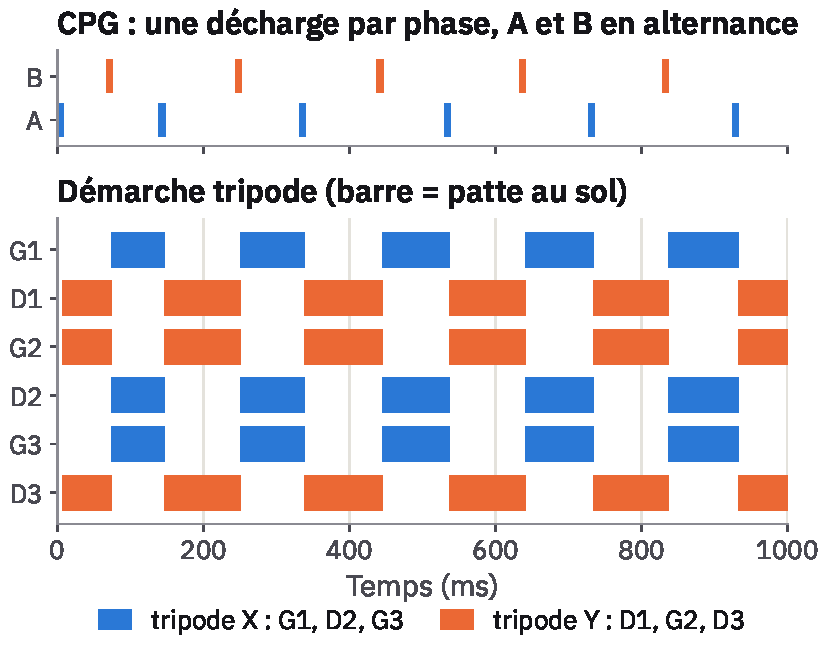
\includegraphics[width=\linewidth]{figures/p1_cpg_demarche}
  \legende{Fig. 1 --- Marche avant.}{A et B alternent, une décharge par phase (période 197~ms à I\_drive = 2). Les deux tripodes se relaient : trois pattes sont toujours au sol.}
  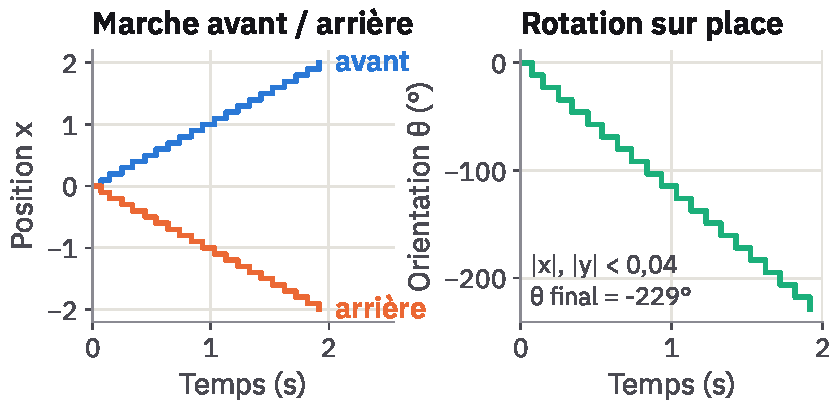
\includegraphics[width=\linewidth]{figures/p1_trajectoires}
  \legende{Fig. 2 --- Même rythme, seul le biais change.}{$x$ = +2,00 en avant et −2,00 en arrière ; θ revient à 0 à chaque cycle, d'où la ligne droite ($y$ = −0,07 : dandinement du tripode). En rotation, $v_G = -v_D$ : θ = −4,0~rad en 2~s et le centre reste en place ($|x|, |y| < 0{,}04$).}
}
\column{0.333}
\block{}{\raggedright%
  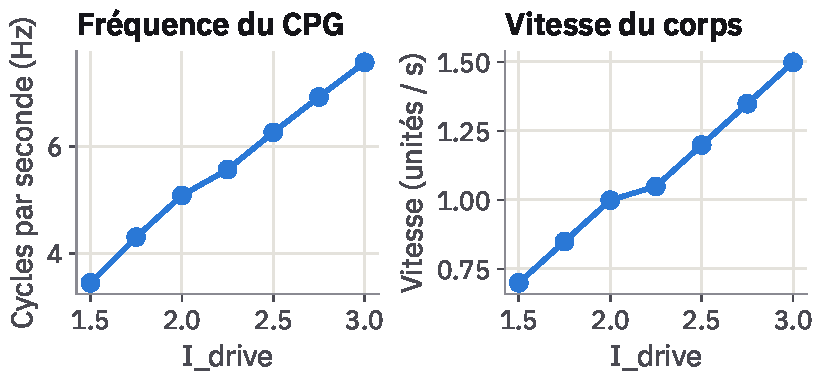
\includegraphics[width=\linewidth]{figures/p1_vitesse}
  \legende{Fig. 3 --- Une seule entrée règle la vitesse.}{De I\_drive = 1,5 à 3 : fréquence 3,4 → 7,6~Hz, vitesse 0,70 → 1,50 unité/s ($\propto$ poussées par seconde).}
  \begin{minipage}[c]{0.42\linewidth}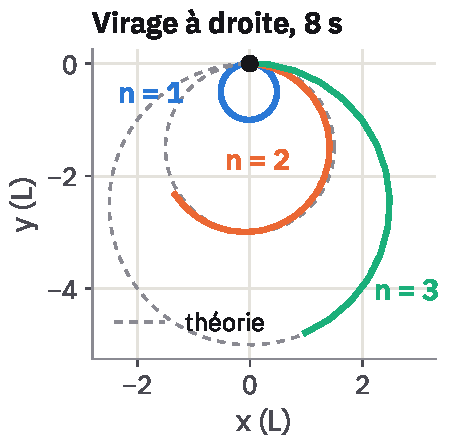
\includegraphics[width=\linewidth]{figures/p1_cercles}\end{minipage}\hfill
  \begin{minipage}[c]{0.54\linewidth}\petit
    \begin{tabularx}{\linewidth}{@{}X r r@{}}
      \toprule
      $n$ & \textbf{R prévu} & \textbf{R mesuré}\\ \midrule
      \code{1} & \code{0,50 L} & \code{0,50 L}\\
      \code{2} & \code{1,50 L} & \code{1,50 L}\\
      \code{3} & \code{2,50 L} & \code{2,55 L}\\ \bottomrule
    \end{tabularx}
  \end{minipage}
  \legende{Fig. 4 --- Cercles.}{Le côté droit saute 1 pas sur $n$ : $v_D = v_G(1 - 1/n)$, d'où $R = (L/2)(2n - 1)$. R mesuré = distance / angle total ; écart ≤ 2~\%.}
  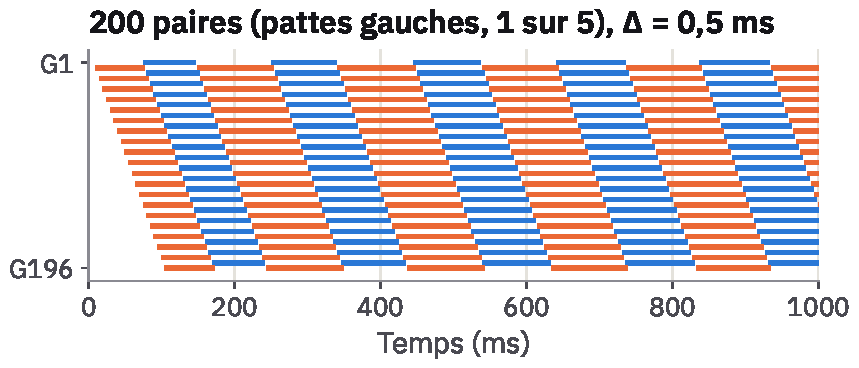
\includegraphics[width=\linewidth]{figures/p1_N200}
  \legende{Fig. 5 --- 200 paires : on ne change que N\_PAIRES.}{La règle $(k + s) \bmod 2$ alterne les segments ; un délai $k\Delta$ crée une onde métachronale de l'avant vers l'arrière. Il reste 4 neurones de virage, quel que soit $N$.}
}
\end{columns}

% ------------------------------------------------------------------ Partie II
\block{}{\bandeau{PARTIE II — SYSTÈME PSEUDO-AUTONOME}}

\begin{columns}
\column{0.333}
\block{}{\raggedright%
  \titre{06}{Des neurones à la place des réglages}
  {\petit Le réseau de la Partie I reste identique ; mode, virage et I\_drive viennent maintenant de neurones de commande pilotés par des capteurs.\par}
  \vspace{4mm}
  \resizebox{\linewidth}{!}{\definecolor{c14805A}{HTML}{14805A}\definecolor{c2A78D6}{HTML}{2A78D6}\definecolor{c6250D6}{HTML}{6250D6}\definecolor{cB9B5AA}{HTML}{B9B5AA}\definecolor{cE1F5EC}{HTML}{E1F5EC}\definecolor{cE3EEFB}{HTML}{E3EEFB}\definecolor{cEB6834}{HTML}{EB6834}\definecolor{cEBE8FB}{HTML}{EBE8FB}\definecolor{cFDE8DF}{HTML}{FDE8DF}\definecolor{cFFFFFF}{HTML}{FFFFFF}
\begin{tikzpicture}[x=0.02646cm, y=-0.02646cm]
\useasboundingbox (0,0) rectangle (942,470);
\draw[bande] (700,24) rectangle (942,464);
\draw[excitl,-{Triangle[length=3.2mm,width=2.6mm]}] (224,84) -- (340,84);
\draw[excitl,-{Triangle[length=3.2mm,width=2.6mm]}] (224,236) -- (340,236);
\draw[excitl,-{Triangle[length=3.2mm,width=2.6mm]}] (224,316) -- (340,316);
\draw[excitl,-{Triangle[length=3.2mm,width=2.6mm]}] (224,416) -- (340,416);
\draw[excitl,-{Triangle[length=3.2mm,width=2.6mm]}] (600,84) -- (716,84);
\draw[excitl,-{Triangle[length=3.2mm,width=2.6mm]}] (600,276) -- (716,276);
\draw[excitl,-{Triangle[length=3.2mm,width=2.6mm]}] (600,416) -- (716,416);
\draw[inhibit,-{Circle[length=2.6mm]}] (470,144) -- (470,199);
\node[carte, fill=cE1F5EC, draw=c14805A, minimum width=5.29cm, minimum height=1.91cm, text width=4.76cm, font=\fontsize{17pt}{20pt}\selectfont] at (124.0,84.0) {\textbf{SENS\_AV}\\{\fontsize{14pt}{16pt}\selectfont contact de face}};
\node[carte, fill=cE3EEFB, draw=c2A78D6, minimum width=5.29cm, minimum height=1.91cm, text width=4.76cm, font=\fontsize{17pt}{20pt}\selectfont] at (124.0,236.0) {\textbf{SENS\_G}\\{\fontsize{14pt}{16pt}\selectfont flanc gauche}};
\node[carte, fill=cFDE8DF, draw=cEB6834, minimum width=5.29cm, minimum height=1.91cm, text width=4.76cm, font=\fontsize{17pt}{20pt}\selectfont] at (124.0,316.0) {\textbf{SENS\_D}\\{\fontsize{14pt}{16pt}\selectfont flanc droit}};
\node[carte, fill=cEBE8FB, draw=c6250D6, minimum width=5.29cm, minimum height=1.91cm, text width=4.76cm, font=\fontsize{17pt}{20pt}\selectfont] at (124.0,416.0) {\textbf{SENS\_AR}\\{\fontsize{14pt}{16pt}\selectfont heurté derrière}};
\node[carte, fill=cFFFFFF, draw=cB9B5AA, minimum width=6.88cm, minimum height=3.18cm, text width=6.35cm, font=\fontsize{16pt}{19pt}\selectfont] at (470.0,84.0) {\textbf{CMD\_AV\_s $\dashv\vdash$ CMD\_AR\_s}\\{\fontsize{14pt}{16pt}\selectfont biais I\_CMD = 1,8 :\\marche avant par défaut}};
\node[carte, fill=cFFFFFF, draw=cB9B5AA, minimum width=6.88cm, minimum height=4.02cm, text width=6.35cm, font=\fontsize{16pt}{19pt}\selectfont] at (470.0,276.0) {\textbf{COMPTEUR\_G / \_D}\\{\fontsize{14pt}{16pt}\selectfont fuite 150 ms ; atteint\\le seuil seulement si\\un flanc est touché}};
\node[carte, fill=cFFFFFF, draw=cB9B5AA, minimum width=6.88cm, minimum height=1.91cm, text width=6.35cm, font=\fontsize{17pt}{20pt}\selectfont] at (470.0,416.0) {\textbf{CPG (A, B)}};
\node[carte, fill=cFFFFFF, draw=cB9B5AA, minimum width=5.56cm, minimum height=10.80cm, text width=5.03cm, font=\fontsize{17pt}{20pt}\selectfont] at (821.0,244.0) {\textbf{Réseau de la Partie I}\\[2mm]{\fontsize{15pt}{17pt}\selectfont biais des IN\\(mode avant / arrière)\\[2mm]INHIB\_s : saute\\1 pas sur n\\[2mm]rythme du CPG\\[2mm]$\rightarrow$ pattes}};
\node[etiq, anchor=north, align=center, text width=2.96cm, font=\fontsize{14pt}{16pt}\selectfont] at (282.0,94.0) {lente\\800 ms};
\node[etiq, anchor=north, align=center, text width=2.96cm, font=\fontsize{14pt}{16pt}\selectfont] at (282.0,248.0) {croisé};
\node[etiq, anchor=north, align=center, text width=2.96cm, font=\fontsize{14pt}{16pt}\selectfont] at (282.0,428.0) {lente};
\node[etiq, anchor=north west, align=left, text width=2.91cm, font=\fontsize{14pt}{16pt}\selectfont] at (484.0,156.0) {AR $\dashv$};
\end{tikzpicture}}\par
  \vspace{5mm}
  {\fontsize{17.5pt}{23.5pt}\selectfont
  \begin{itemize}[label={}]
    \item \textbf{Capteurs.} 4 groupes de 10 neurones aux seuils 0,2 à 1,8 : un contact plus fort recrute plus de neurones, qui déchargent plus vite \cite[§2.1]{porcino1990}.
    \item \textbf{Commandes.} CMD\_AV reçoit un biais (I\_CMD = 1,8) : marche avant par défaut. CMD\_AV $\dashv\vdash$ CMD\_AR (gagnant-prend-tout) ; un contact de face excite CMD\_AR et inhibe CMD\_AV \cite[p.~1437]{cruse1998}.
    \item \textbf{Persistance.} Synapses lentes ($\tau_{\mathrm{persist}}$ = 800~ms) : la réaction dure plus longtemps que le contact.
    \item \textbf{Virages gradués.} Un flanc touché pousse le COMPTEUR opposé au seuil : plus le contact est fort, plus il saute de pas ; fort, il active aussi CMD\_AR : pivot \cite[p.~112--113]{otis2004}.
    \item \textbf{Hiérarchie.} Inhibition entre capteurs : avant > flancs > arrière ; entre G et D, le plus fort gagne \cite[p.~1436]{cruse1998}.
  \end{itemize}}
}
\column{0.333}
\block{}{\raggedright%
  \titre{07}{Résultats}
  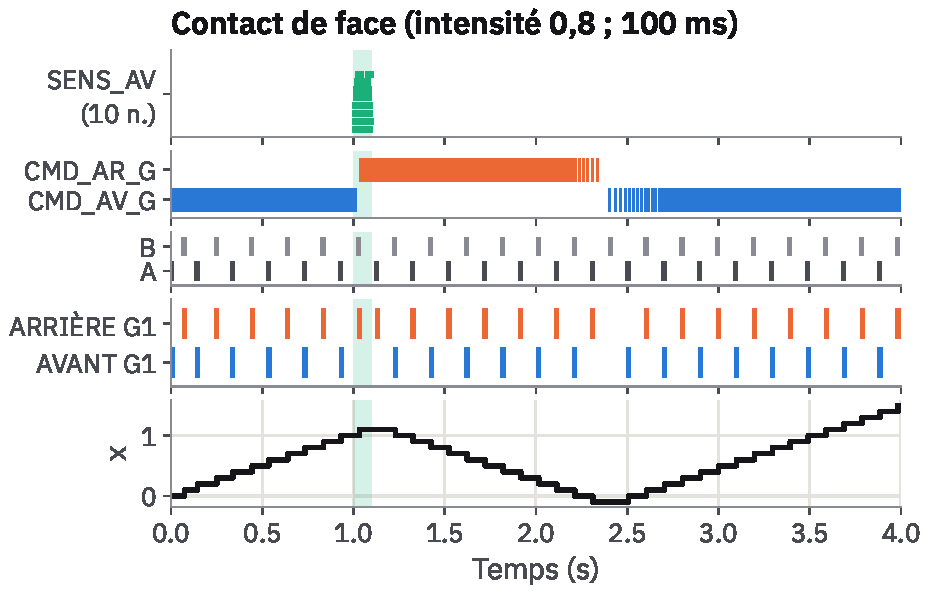
\includegraphics[width=\linewidth]{figures/p2_raster_recul}
  \legende{Fig. 6 --- Obstacle de face → reculer.}{SENS\_AV fait basculer CMD\_AV\_G vers CMD\_AR\_G 36~ms après le contact. Le CPG ne change pas : seuls AVANT et ARRIÈRE s'inversent. L'hexapode recule de 1,2 unité pendant 1,3~s, puis CMD\_AV reprend la main et la marche avant repart.}
  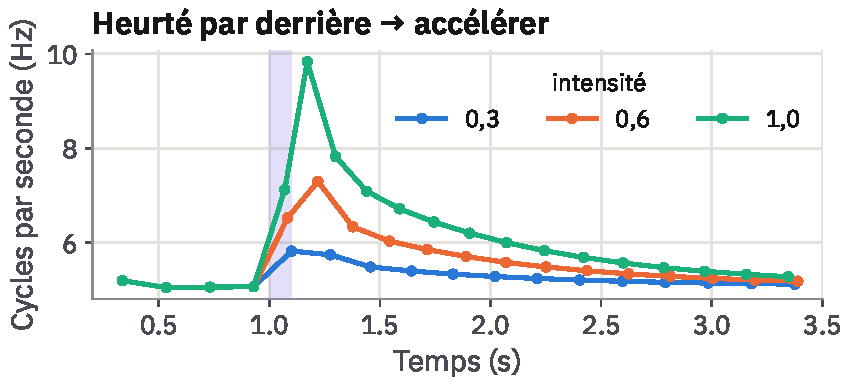
\includegraphics[width=\linewidth]{figures/p2_acceleration}
  \legende{Fig. 7 --- Heurté par derrière → accélérer.}{SENS\_AR excite A et B par une synapse lente : la fréquence passe de 5,1~Hz à 5,8, 7,3 ou 9,8~Hz (intensité 0,3, 0,6 ou 1,0), puis redescend progressivement vers 5,1~Hz.}
}
\column{0.333}
\block{}{\raggedright%
  \centering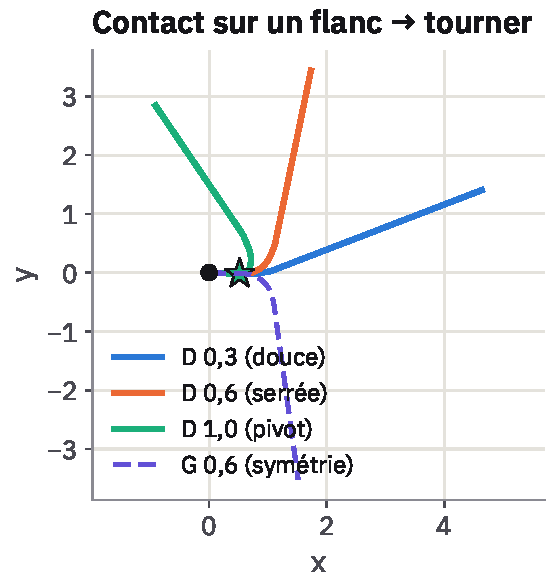
\includegraphics[width=0.6\linewidth]{figures/p2_virages}\par\raggedright
  \legende{Fig. 8 --- Obstacle sur un flanc → tourner du côté opposé.}{Contact à droite à 0,5~s (étoile) : faible (0,3), courbe douce, θ = +19° ; moyen (0,6), virage serré, +76° ; fort (1,0), CMD\_AR\_G s'active : pivot, +122°. Le contact à gauche (0,6) donne le virage miroir (−84°).}
  \encadre{\fontsize{17pt}{22pt}\selectfont\textbf{Adapter le comportement par les paramètres (annexe)}\par\vspace{2mm}
    \begin{tabularx}{\linewidth}{@{}>{\ttfamily}l X@{}}
      W\_AV\_AR & intensité minimale pour reculer (sensibilité)\\
      $\tau$\_persist & durée de la réaction\\
      DELAI\_SENS & temps de réaction (distance avant de reculer)\\
      W\_LAT\_AR & intensité où le virage devient un pivot\\
      seuils capteurs & plage d'intensités distinguées\\
    \end{tabularx}\par\vspace{2mm}
    {\color{encre2}Bonus (code seulement, \code{exp\_part2\_stimuli habituation arene}) : boucle fermée dans une arène, où l'hexapode réagit seul aux murs ; habituation de l'accélération aux poussées répétées.}}
}
\end{columns}

% ------------------------------------------------------------------ Discussion
\block{}{\noindent\leaders\hrule height 1.2mm\hfill\null}
\begin{columns}
\column{0.666}
\block{}{\raggedright%
  \titre{08}{Discussion}
  \begin{minipage}[t]{0.48\linewidth}\fontsize{17.5pt}{23.5pt}\selectfont
    \textbf{Ce qui fonctionne}\par\vspace{2mm}
    Un seul métronome sert à toutes les tâches : direction, rotation et virage ne font que moduler (biais, inhibition) le même rythme, comme le CPG biologique \cite{otis2004}. Passer à 200 paires ne touche qu'une variable, et les neurones de commande ne dépendent pas de $N$. Les prédictions tiennent : $R = (L/2)(2n - 1)$ à 2~\% près, vitesse proportionnelle à la fréquence. En Partie II, les capteurs modifient le rythme sans le remplacer.
  \end{minipage}\hfill
  \begin{minipage}[t]{0.48\linewidth}\fontsize{17.5pt}{23.5pt}\selectfont
    \textbf{Limites et pistes}\par\vspace{2mm}
    Pas de rétroaction des pattes : le rythme est imposé, sans capteurs de charge ou de position comme chez Beer \cite{beer1992} et Cruse \cite{cruse1998}. Le virage procède par pas entiers sautés, et la durée du blocage (≈ 149~ms) est réglée pour I\_drive ≈ 2 au lieu de suivre la fréquence ; un blocage déclenché par B s'y adapterait. La cinématique est simplifiée (poussée = déplacement fixe $d$). Les poids de la Partie II sont réglés à la main ; un apprentissage (STDP) est une suite naturelle.
  \end{minipage}
}
\column{0.333}
\block{}{\raggedright%
  {\condensed\fontsize{30pt}{34pt}\selectfont Références}\par\vspace{2mm}
  {\fontsize{12.5pt}{15.5pt}\selectfont
  \makeatletter\renewcommand\section[2]{}\makeatother
  \bibliographystyle{unsrt}
  \bibliography{references}\par}
}
\end{columns}

\end{document}
